\documentclass[1p]{elsarticle_modified}
%\bibliographystyle{elsarticle-num}

%\usepackage[colorlinks]{hyperref}
%\usepackage{abbrmath_seonhwa} %\Abb, \Ascr, \Acal ,\Abf, \Afrak
\usepackage{amsfonts}
\usepackage{amssymb}
\usepackage{amsmath}
\usepackage{amsthm}
\usepackage{scalefnt}
\usepackage{amsbsy}
\usepackage{kotex}
\usepackage{caption}
\usepackage{subfig}
\usepackage{color}
\usepackage{graphicx}
\usepackage{xcolor} %% white, black, red, green, blue, cyan, magenta, yellow
\usepackage{float}
\usepackage{setspace}
\usepackage{hyperref}

\usepackage{tikz}
\usetikzlibrary{arrows}

\usepackage{multirow}
\usepackage{array} % fixed length table
\usepackage{hhline}

%%%%%%%%%%%%%%%%%%%%%
\makeatletter
\renewcommand*\env@matrix[1][\arraystretch]{%
	\edef\arraystretch{#1}%
	\hskip -\arraycolsep
	\let\@ifnextchar\new@ifnextchar
	\array{*\c@MaxMatrixCols c}}
\makeatother %https://tex.stackexchange.com/questions/14071/how-can-i-increase-the-line-spacing-in-a-matrix
%%%%%%%%%%%%%%%

\usepackage[normalem]{ulem}

\newcommand{\msout}[1]{\ifmmode\text{\sout{\ensuremath{#1}}}\else\sout{#1}\fi}
%SOURCE: \msout is \stkout macro in https://tex.stackexchange.com/questions/20609/strikeout-in-math-mode

\newcommand{\cancel}[1]{
	\ifmmode
	{\color{red}\msout{#1}}
	\else
	{\color{red}\sout{#1}}
	\fi
}

\newcommand{\add}[1]{
	{\color{blue}\uwave{#1}}
}

\newcommand{\replace}[2]{
	\ifmmode
	{\color{red}\msout{#1}}{\color{blue}\uwave{#2}}
	\else
	{\color{red}\sout{#1}}{\color{blue}\uwave{#2}}
	\fi
}

\newcommand{\Sol}{\mathcal{S}} %segment
\newcommand{\D}{D} %diagram
\newcommand{\A}{\mathcal{A}} %arc


%%%%%%%%%%%%%%%%%%%%%%%%%%%%%5 test

\def\sl{\operatorname{\textup{SL}}(2,\Cbb)}
\def\psl{\operatorname{\textup{PSL}}(2,\Cbb)}
\def\quan{\mkern 1mu \triangleright \mkern 1mu}

\theoremstyle{definition}
\newtheorem{thm}{Theorem}[section]
\newtheorem{prop}[thm]{Proposition}
\newtheorem{lem}[thm]{Lemma}
\newtheorem{ques}[thm]{Question}
\newtheorem{cor}[thm]{Corollary}
\newtheorem{defn}[thm]{Definition}
\newtheorem{exam}[thm]{Example}
\newtheorem{rmk}[thm]{Remark}
\newtheorem{alg}[thm]{Algorithm}

\newcommand{\I}{\sqrt{-1}}
\begin{document}

%\begin{frontmatter}
%
%\title{Boundary parabolic representations of knots up to 8 crossings}
%
%%% Group authors per affiliation:
%\author{Yunhi Cho} 
%\address{Department of Mathematics, University of Seoul, Seoul, Korea}
%\ead{yhcho@uos.ac.kr}
%
%
%\author{Seonhwa Kim} %\fnref{s_kim}}
%\address{Center for Geometry and Physics, Institute for Basic Science, Pohang, 37673, Korea}
%\ead{ryeona17@ibs.re.kr}
%
%\author{Hyuk Kim}
%\address{Department of Mathematical Sciences, Seoul National University, Seoul 08826, Korea}
%\ead{hyukkim@snu.ac.kr}
%
%\author{Seokbeom Yoon}
%\address{Department of Mathematical Sciences, Seoul National University, Seoul, 08826,  Korea}
%\ead{sbyoon15@snu.ac.kr}
%
%\begin{abstract}
%We find all boundary parabolic representation of knots up to 8 crossings.
%
%\end{abstract}
%\begin{keyword}
%    \MSC[2010] 57M25 
%\end{keyword}
%
%\end{frontmatter}

%\linenumbers
%\tableofcontents
%
\newcommand\colored[1]{\textcolor{white}{\rule[-0.35ex]{0.8em}{1.4ex}}\kern-0.8em\color{red} #1}%
%\newcommand\colored[1]{\textcolor{white}{ #1}\kern-2.17ex	\textcolor{white}{ #1}\kern-1.81ex	\textcolor{white}{ #1}\kern-2.15ex\color{red}#1	}

{\Large $\underline{11n_{12}~(K11n_{12})}$}

\setlength{\tabcolsep}{10pt}
\renewcommand{\arraystretch}{1.6}
\vspace{1cm}\begin{tabular}{m{100pt}>{\centering\arraybackslash}m{274pt}}
\multirow{5}{120pt}{
	\centering
	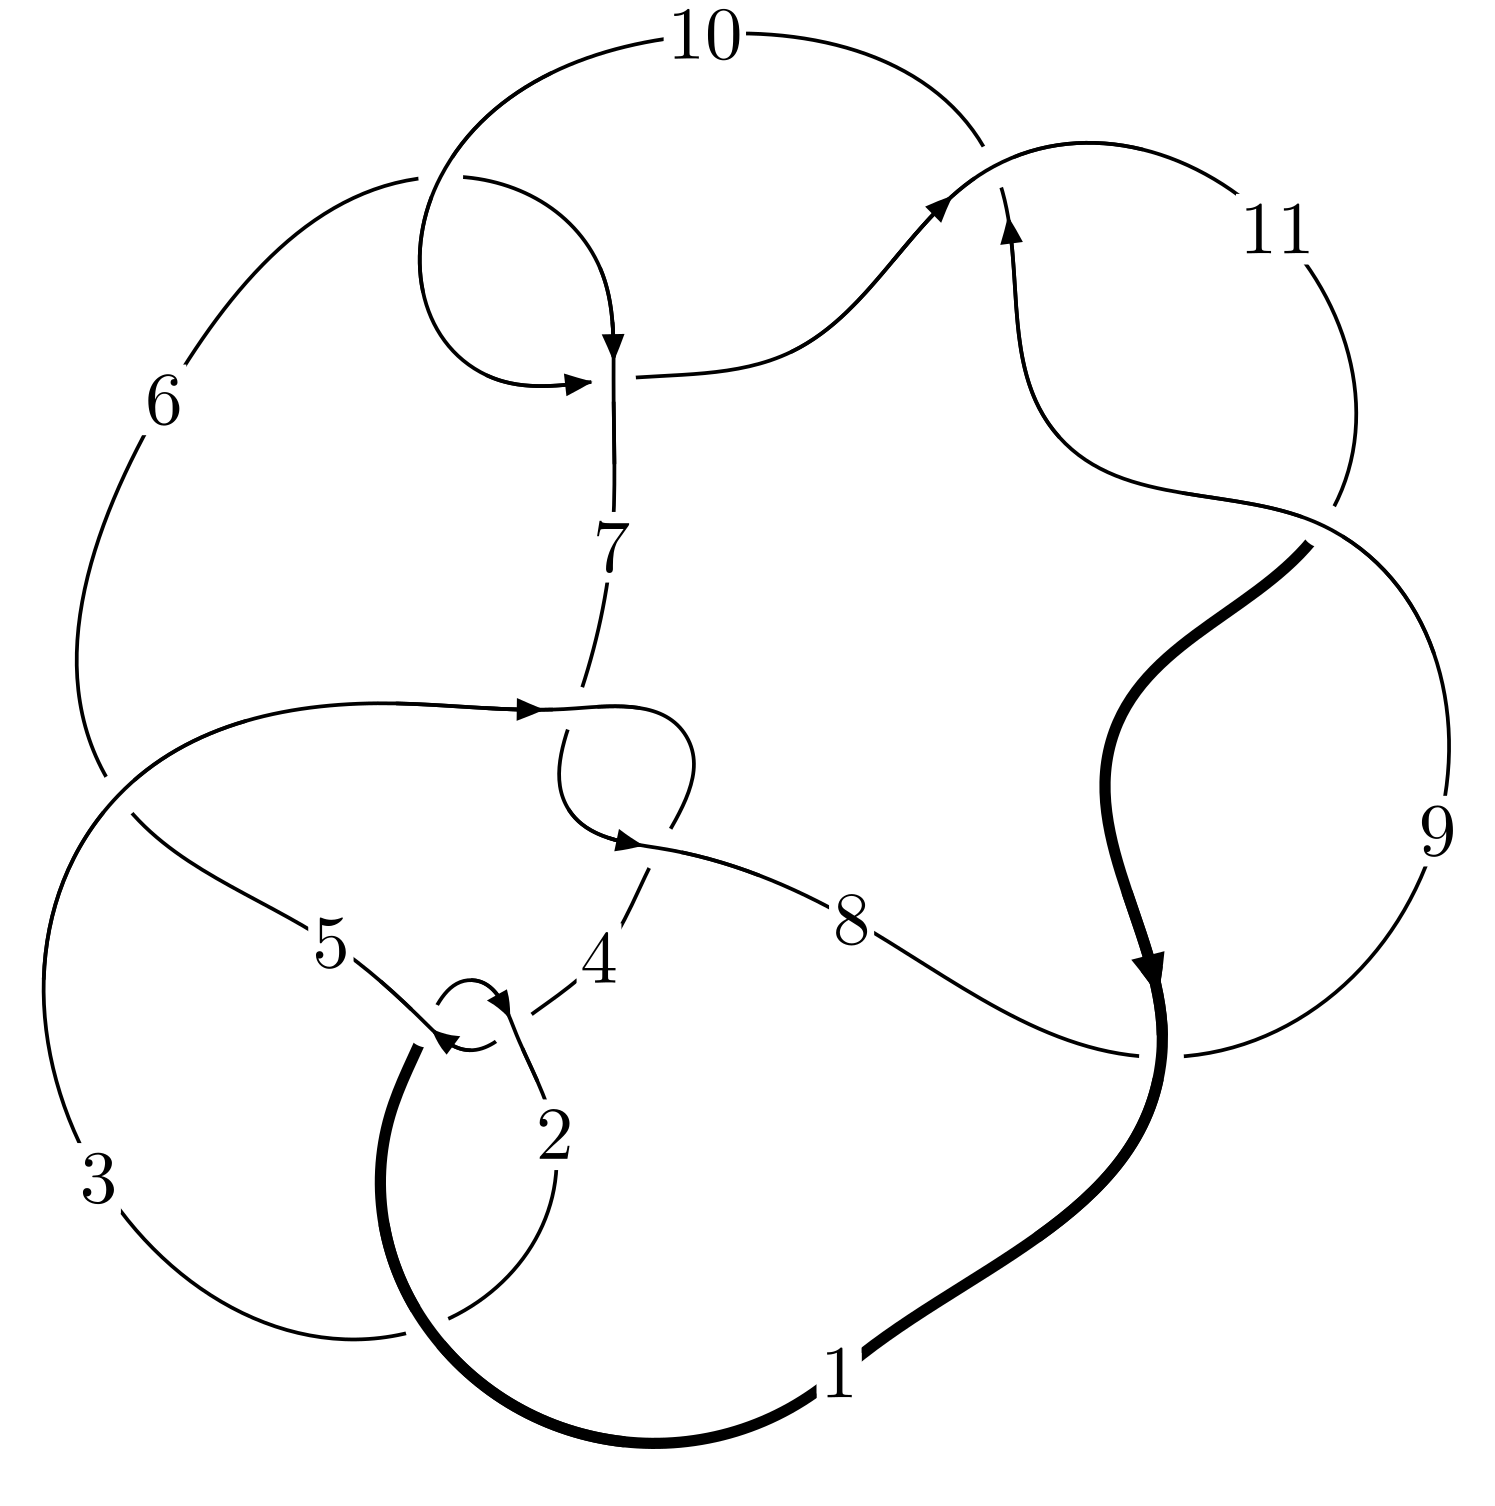
\includegraphics[width=112pt]{../../../GIT/diagram.site/Diagrams/png/628_11n_12.png}\\
\ \ \ A knot diagram\footnotemark}&
\allowdisplaybreaks
\textbf{Linearized knot diagam} \\
\cline{2-2}
 &
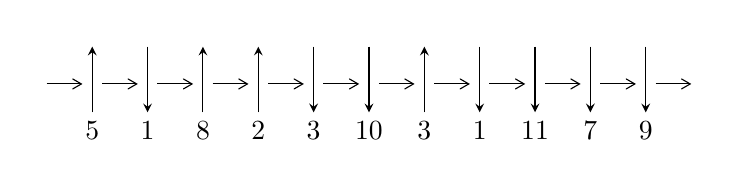
\begin{tikzpicture}[x=20pt, y=17pt]
	% nodes
	\node (C0) at (0, 0) {};
	\node (C1) at (1, 0) {};
	\node (C1U) at (1, +1) {};
	\node (C1D) at (1, -1) {5};

	\node (C2) at (2, 0) {};
	\node (C2U) at (2, +1) {};
	\node (C2D) at (2, -1) {1};

	\node (C3) at (3, 0) {};
	\node (C3U) at (3, +1) {};
	\node (C3D) at (3, -1) {8};

	\node (C4) at (4, 0) {};
	\node (C4U) at (4, +1) {};
	\node (C4D) at (4, -1) {2};

	\node (C5) at (5, 0) {};
	\node (C5U) at (5, +1) {};
	\node (C5D) at (5, -1) {3};

	\node (C6) at (6, 0) {};
	\node (C6U) at (6, +1) {};
	\node (C6D) at (6, -1) {10};

	\node (C7) at (7, 0) {};
	\node (C7U) at (7, +1) {};
	\node (C7D) at (7, -1) {3};

	\node (C8) at (8, 0) {};
	\node (C8U) at (8, +1) {};
	\node (C8D) at (8, -1) {1};

	\node (C9) at (9, 0) {};
	\node (C9U) at (9, +1) {};
	\node (C9D) at (9, -1) {11};

	\node (C10) at (10, 0) {};
	\node (C10U) at (10, +1) {};
	\node (C10D) at (10, -1) {7};

	\node (C11) at (11, 0) {};
	\node (C11U) at (11, +1) {};
	\node (C11D) at (11, -1) {9};
	\node (C12) at (12, 0) {};

	% arrows
	\draw[->,>={angle 60}]
	(C0) edge (C1) (C1) edge (C2) (C2) edge (C3) (C3) edge (C4) (C4) edge (C5) (C5) edge (C6) (C6) edge (C7) (C7) edge (C8) (C8) edge (C9) (C9) edge (C10) (C10) edge (C11) (C11) edge (C12) ;	\draw[->,>=stealth]
	(C1D) edge (C1U) (C2U) edge (C2D) (C3D) edge (C3U) (C4D) edge (C4U) (C5U) edge (C5D) (C6U) edge (C6D) (C7D) edge (C7U) (C8U) edge (C8D) (C9U) edge (C9D) (C10U) edge (C10D) (C11U) edge (C11D) ;
	\end{tikzpicture} \\
\hhline{~~} \\& 
\textbf{Solving Sequence} \\ \cline{2-2} 
 &
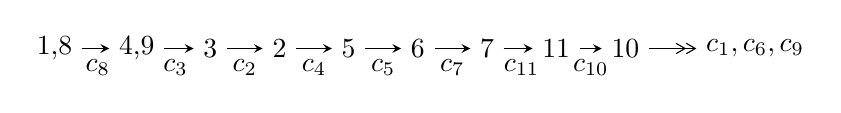
\begin{tikzpicture}[x=25pt, y=7pt]
	% node
	\node (A0) at (-1/8, 0) {1,8};
	\node (A1) at (17/16, 0) {4,9};
	\node (A2) at (17/8, 0) {3};
	\node (A3) at (25/8, 0) {2};
	\node (A4) at (33/8, 0) {5};
	\node (A5) at (41/8, 0) {6};
	\node (A6) at (49/8, 0) {7};
	\node (A7) at (57/8, 0) {11};
	\node (A8) at (65/8, 0) {10};
	\node (C1) at (1/2, -1) {$c_{8}$};
	\node (C2) at (13/8, -1) {$c_{3}$};
	\node (C3) at (21/8, -1) {$c_{2}$};
	\node (C4) at (29/8, -1) {$c_{4}$};
	\node (C5) at (37/8, -1) {$c_{5}$};
	\node (C6) at (45/8, -1) {$c_{7}$};
	\node (C7) at (53/8, -1) {$c_{11}$};
	\node (C8) at (61/8, -1) {$c_{10}$};
	\node (A9) at (10, 0) {$c_{1},c_{6},c_{9}$};

	% edge
	\draw[->,>=stealth]	
	(A0) edge (A1) (A1) edge (A2) (A2) edge (A3) (A3) edge (A4) (A4) edge (A5) (A5) edge (A6) (A6) edge (A7) (A7) edge (A8) ;
	\draw[->>,>={angle 60}]	
	(A8) edge (A9);
\end{tikzpicture} \\ 

\end{tabular} \\

\footnotetext{
The image of knot diagram is generated by the software ``\textbf{Draw programme}" developed by Andrew Bartholomew(\url{http://www.layer8.co.uk/maths/draw/index.htm\#Running-draw}), where we modified some parts for our purpose(\url{https://github.com/CATsTAILs/LinksPainter}).
}\phantom \\ \newline 
\centering \textbf{Ideals for irreducible components\footnotemark of $X_{\text{par}}$} 
 
\begin{align*}
I^u_{1}&=\langle 
-4 u^{11}-85 u^{10}+\cdots+8858 b-4180,\;-5021 u^{11}+9565 u^{10}+\cdots+17716 a+23565,\\
\phantom{I^u_{1}}&\phantom{= \langle  }u^{12}- u^{11}+12 u^{10}-11 u^9+47 u^8-37 u^7+56 u^6-30 u^5-12 u^4+12 u^3- u+1\rangle \\
I^u_{2}&=\langle 
b,\;u^2 a+a^2- a u+2 u^2+2 a- u+3,\;u^3- u^2+2 u-1\rangle \\
\\
\end{align*}
\raggedright * 2 irreducible components of $\dim_{\mathbb{C}}=0$, with total 18 representations.\\
\footnotetext{All coefficients of polynomials are rational numbers. But the coefficients are sometimes approximated in decimal forms when there is not enough margin.}
\newpage
\renewcommand{\arraystretch}{1}
\centering \section*{I. $I^u_{1}= \langle -4 u^{11}-85 u^{10}+\cdots+8858 b-4180,\;-5021 u^{11}+9565 u^{10}+\cdots+17716 a+23565,\;u^{12}- u^{11}+\cdots- u+1 \rangle$}
\flushleft \textbf{(i) Arc colorings}\\
\begin{tabular}{m{7pt} m{180pt} m{7pt} m{180pt} }
\flushright $a_{1}=$&$\begin{pmatrix}0\\u\end{pmatrix}$ \\
\flushright $a_{8}=$&$\begin{pmatrix}1\\0\end{pmatrix}$ \\
\flushright $a_{4}=$&$\begin{pmatrix}0.283416 u^{11}-0.539907 u^{10}+\cdots+0.840596 u-1.33015\\0.000451569 u^{11}+0.00959585 u^{10}+\cdots+0.903251 u+0.471890\end{pmatrix}$ \\
\flushright $a_{9}=$&$\begin{pmatrix}1\\u^2\end{pmatrix}$ \\
\flushright $a_{3}=$&$\begin{pmatrix}0.282965 u^{11}-0.549503 u^{10}+\cdots-0.0626552 u-1.80204\\0.000451569 u^{11}+0.00959585 u^{10}+\cdots+0.903251 u+0.471890\end{pmatrix}$ \\
\flushright $a_{2}=$&$\begin{pmatrix}0.282965 u^{11}-0.549503 u^{10}+\cdots-0.0626552 u-1.80204\\0.0559381 u^{11}+0.00118537 u^{10}+\cdots+1.45275 u+0.205351\end{pmatrix}$ \\
\flushright $a_{5}=$&$\begin{pmatrix}-0.658106 u^{11}+0.452755 u^{10}+\cdots-1.93836 u-0.720422\\u\end{pmatrix}$ \\
\flushright $a_{6}=$&$\begin{pmatrix}0.00203206 u^{11}-0.206819 u^{10}+\cdots-2.18537 u+1.12350\\0.207496 u^{11}-0.340709 u^{10}+\cdots-1.20603 u+0.333371\end{pmatrix}$ \\
\flushright $a_{7}=$&$\begin{pmatrix}-0.128584 u^{11}+0.142583 u^{10}+\cdots+1.17419 u-0.870625\\-0.204787 u^{11}+0.398284 u^{10}+\cdots+1.12554 u-0.00203206\end{pmatrix}$ \\
\flushright $a_{11}=$&$\begin{pmatrix}u\\u^3+u\end{pmatrix}$ \\
\flushright $a_{10}=$&$\begin{pmatrix}u^2+1\\u^4+2 u^2\end{pmatrix}$\\ \flushright $a_{10}=$&$\begin{pmatrix}u^2+1\\u^4+2 u^2\end{pmatrix}$\\&\end{tabular}
\flushleft \textbf{(ii) Obstruction class $= -1$}\\~\\
\flushleft \textbf{(iii) Cusp Shapes $= \frac{56005}{17716} u^{11}-\frac{11673}{4429} u^{10}+\frac{166280}{4429} u^9-\frac{127032}{4429} u^8+\frac{2558331}{17716} u^7-\frac{418885}{4429} u^6+\frac{726025}{4429} u^5-\frac{1302141}{17716} u^4-\frac{815229}{17716} u^3+\frac{405337}{17716} u^2+\frac{46603}{8858} u-\frac{28579}{8858}$}\\~\\
\newpage\renewcommand{\arraystretch}{1}
\flushleft \textbf{(iv) u-Polynomials at the component}\newline \\
\begin{tabular}{m{50pt}|m{274pt}}
Crossings & \hspace{64pt}u-Polynomials at each crossing \\
\hline $$\begin{aligned}c_{1},c_{4}\end{aligned}$$&$\begin{aligned}
&u^{12}+4 u^{11}+\cdots+2 u+1
\end{aligned}$\\
\hline $$\begin{aligned}c_{2}\end{aligned}$$&$\begin{aligned}
&u^{12}+14 u^{10}+\cdots+10 u+1
\end{aligned}$\\
\hline $$\begin{aligned}c_{3},c_{7}\end{aligned}$$&$\begin{aligned}
&u^{12}+u^{11}+\cdots+288 u+64
\end{aligned}$\\
\hline $$\begin{aligned}c_{5}\end{aligned}$$&$\begin{aligned}
&u^{12}-4 u^{11}+\cdots+532 u+193
\end{aligned}$\\
\hline $$\begin{aligned}c_{6},c_{10}\end{aligned}$$&$\begin{aligned}
&u^{12}+3 u^{11}+4 u^{10}+u^9+u^8+7 u^7+12 u^6+6 u^5+u+1
\end{aligned}$\\
\hline $$\begin{aligned}c_{8},c_{9},c_{11}\end{aligned}$$&$\begin{aligned}
&u^{12}+u^{11}+\cdots+u+1
\end{aligned}$\\
\hline
\end{tabular}\\~\\
\newpage\renewcommand{\arraystretch}{1}
\flushleft \textbf{(v) Riley Polynomials at the component}\newline \\
\begin{tabular}{m{50pt}|m{274pt}}
Crossings & \hspace{64pt}Riley Polynomials at each crossing \\
\hline $$\begin{aligned}c_{1},c_{4}\end{aligned}$$&$\begin{aligned}
&y^{12}+14 y^{10}+\cdots+10 y+1
\end{aligned}$\\
\hline $$\begin{aligned}c_{2}\end{aligned}$$&$\begin{aligned}
&y^{12}+28 y^{11}+\cdots-66 y+1
\end{aligned}$\\
\hline $$\begin{aligned}c_{3},c_{7}\end{aligned}$$&$\begin{aligned}
&y^{12}-35 y^{11}+\cdots-9216 y+4096
\end{aligned}$\\
\hline $$\begin{aligned}c_{5}\end{aligned}$$&$\begin{aligned}
&y^{12}+56 y^{11}+\cdots+602074 y+37249
\end{aligned}$\\
\hline $$\begin{aligned}c_{6},c_{10}\end{aligned}$$&$\begin{aligned}
&y^{12}- y^{11}+\cdots- y+1
\end{aligned}$\\
\hline $$\begin{aligned}c_{8},c_{9},c_{11}\end{aligned}$$&$\begin{aligned}
&y^{12}+23 y^{11}+\cdots- y+1
\end{aligned}$\\
\hline
\end{tabular}\\~\\
\newpage\flushleft \textbf{(vi) Complex Volumes and Cusp Shapes}
$$\begin{array}{c|c|c}  
\text{Solutions to }I^u_{1}& \I (\text{vol} + \sqrt{-1}CS) & \text{Cusp shape}\\
 \hline 
\begin{aligned}
u &= \phantom{-}0.625204 + 0.231089 I \\
a &= \phantom{-}0.161222 + 0.490070 I \\
b &= \phantom{-}0.412005 + 0.431173 I\end{aligned}
 & -1.40636 - 0.34980 I & -7.54487 + 0.48017 I \\ \hline\begin{aligned}
u &= \phantom{-}0.625204 - 0.231089 I \\
a &= \phantom{-}0.161222 - 0.490070 I \\
b &= \phantom{-}0.412005 - 0.431173 I\end{aligned}
 & -1.40636 + 0.34980 I & -7.54487 - 0.48017 I \\ \hline\begin{aligned}
u &= -0.449650 + 0.155107 I \\
a &= -1.84569 + 2.79630 I \\
b &= -0.674003 + 1.032060 I\end{aligned}
 & \phantom{-}1.31906 - 1.56861 I & \phantom{-}1.73907 + 2.71444 I \\ \hline\begin{aligned}
u &= -0.449650 - 0.155107 I \\
a &= -1.84569 - 2.79630 I \\
b &= -0.674003 - 1.032060 I\end{aligned}
 & \phantom{-}1.31906 + 1.56861 I & \phantom{-}1.73907 - 2.71444 I \\ \hline\begin{aligned}
u &= \phantom{-}0.170188 + 0.372008 I \\
a &= -1.72486 + 0.94221 I \\
b &= \phantom{-}0.737368 - 0.073970 I\end{aligned}
 & -0.55164 - 2.71818 I & -0.33339 + 6.77292 I \\ \hline\begin{aligned}
u &= \phantom{-}0.170188 - 0.372008 I \\
a &= -1.72486 - 0.94221 I \\
b &= \phantom{-}0.737368 + 0.073970 I\end{aligned}
 & -0.55164 + 2.71818 I & -0.33339 - 6.77292 I \\ \hline\begin{aligned}
u &= \phantom{-}0.18845 + 1.62161 I \\
a &= \phantom{-}0.231111 + 0.902812 I \\
b &= \phantom{-}0.359686 + 1.355750 I\end{aligned}
 & \phantom{-}4.35182 - 3.22757 I & \phantom{-}0.42641 + 2.31513 I \\ \hline\begin{aligned}
u &= \phantom{-}0.18845 - 1.62161 I \\
a &= \phantom{-}0.231111 - 0.902812 I \\
b &= \phantom{-}0.359686 - 1.355750 I\end{aligned}
 & \phantom{-}4.35182 + 3.22757 I & \phantom{-}0.42641 - 2.31513 I \\ \hline\begin{aligned}
u &= -0.19909 + 2.16177 I \\
a &= -2.12976 - 0.49437 I \\
b &= -3.33668 - 0.28827 I\end{aligned}
 & -18.9549 + 0.4085 I & \phantom{-}0.320898 + 0.107074 I \\ \hline\begin{aligned}
u &= -0.19909 - 2.16177 I \\
a &= -2.12976 + 0.49437 I \\
b &= -3.33668 + 0.28827 I\end{aligned}
 & -18.9549 - 0.4085 I & \phantom{-}0.320898 - 0.107074 I\\
 \hline 
 \end{array}$$\newpage$$\begin{array}{c|c|c}  
\text{Solutions to }I^u_{1}& \I (\text{vol} + \sqrt{-1}CS) & \text{Cusp shape}\\
 \hline 
\begin{aligned}
u &= \phantom{-}0.16491 + 2.16925 I \\
a &= \phantom{-}1.80797 - 0.87122 I \\
b &= \phantom{-}3.00162 - 0.87325 I\end{aligned}
 & -19.3015 - 8.0703 I & -0.10811 + 3.87488 I \\ \hline\begin{aligned}
u &= \phantom{-}0.16491 - 2.16925 I \\
a &= \phantom{-}1.80797 + 0.87122 I \\
b &= \phantom{-}3.00162 + 0.87325 I\end{aligned}
 & -19.3015 + 8.0703 I & -0.10811 - 3.87488 I\\
 \hline 
 \end{array}$$\newpage\newpage\renewcommand{\arraystretch}{1}
\centering \section*{II. $I^u_{2}= \langle b,\;u^2 a+a^2- a u+2 u^2+2 a- u+3,\;u^3- u^2+2 u-1 \rangle$}
\flushleft \textbf{(i) Arc colorings}\\
\begin{tabular}{m{7pt} m{180pt} m{7pt} m{180pt} }
\flushright $a_{1}=$&$\begin{pmatrix}0\\u\end{pmatrix}$ \\
\flushright $a_{8}=$&$\begin{pmatrix}1\\0\end{pmatrix}$ \\
\flushright $a_{4}=$&$\begin{pmatrix}a\\0\end{pmatrix}$ \\
\flushright $a_{9}=$&$\begin{pmatrix}1\\u^2\end{pmatrix}$ \\
\flushright $a_{3}=$&$\begin{pmatrix}a\\0\end{pmatrix}$ \\
\flushright $a_{2}=$&$\begin{pmatrix}a\\- u^2 a\end{pmatrix}$ \\
\flushright $a_{5}=$&$\begin{pmatrix}u^2+a- u+2\\- u\end{pmatrix}$ \\
\flushright $a_{6}=$&$\begin{pmatrix}0\\- u\end{pmatrix}$ \\
\flushright $a_{7}=$&$\begin{pmatrix}1\\0\end{pmatrix}$ \\
\flushright $a_{11}=$&$\begin{pmatrix}u\\u^2- u+1\end{pmatrix}$ \\
\flushright $a_{10}=$&$\begin{pmatrix}u^2+1\\u^2- u+1\end{pmatrix}$\\ \flushright $a_{10}=$&$\begin{pmatrix}u^2+1\\u^2- u+1\end{pmatrix}$\\&\end{tabular}
\flushleft \textbf{(ii) Obstruction class $= 1$}\\~\\
\flushleft \textbf{(iii) Cusp Shapes $= -3 a u-2 u^2+a+3 u-7$}\\~\\
\newpage\renewcommand{\arraystretch}{1}
\flushleft \textbf{(iv) u-Polynomials at the component}\newline \\
\begin{tabular}{m{50pt}|m{274pt}}
Crossings & \hspace{64pt}u-Polynomials at each crossing \\
\hline $$\begin{aligned}c_{1},c_{2},c_{5}\end{aligned}$$&$\begin{aligned}
&(u^2+u+1)^3
\end{aligned}$\\
\hline $$\begin{aligned}c_{3},c_{7}\end{aligned}$$&$\begin{aligned}
&u^6
\end{aligned}$\\
\hline $$\begin{aligned}c_{4}\end{aligned}$$&$\begin{aligned}
&(u^2- u+1)^3
\end{aligned}$\\
\hline $$\begin{aligned}c_{6}\end{aligned}$$&$\begin{aligned}
&(u^3+u^2-1)^2
\end{aligned}$\\
\hline $$\begin{aligned}c_{8},c_{9}\end{aligned}$$&$\begin{aligned}
&(u^3- u^2+2 u-1)^2
\end{aligned}$\\
\hline $$\begin{aligned}c_{10}\end{aligned}$$&$\begin{aligned}
&(u^3- u^2+1)^2
\end{aligned}$\\
\hline $$\begin{aligned}c_{11}\end{aligned}$$&$\begin{aligned}
&(u^3+u^2+2 u+1)^2
\end{aligned}$\\
\hline
\end{tabular}\\~\\
\newpage\renewcommand{\arraystretch}{1}
\flushleft \textbf{(v) Riley Polynomials at the component}\newline \\
\begin{tabular}{m{50pt}|m{274pt}}
Crossings & \hspace{64pt}Riley Polynomials at each crossing \\
\hline $$\begin{aligned}c_{1},c_{2},c_{4}\\c_{5}\end{aligned}$$&$\begin{aligned}
&(y^2+y+1)^3
\end{aligned}$\\
\hline $$\begin{aligned}c_{3},c_{7}\end{aligned}$$&$\begin{aligned}
&y^6
\end{aligned}$\\
\hline $$\begin{aligned}c_{6},c_{10}\end{aligned}$$&$\begin{aligned}
&(y^3- y^2+2 y-1)^2
\end{aligned}$\\
\hline $$\begin{aligned}c_{8},c_{9},c_{11}\end{aligned}$$&$\begin{aligned}
&(y^3+3 y^2+2 y-1)^2
\end{aligned}$\\
\hline
\end{tabular}\\~\\
\newpage\flushleft \textbf{(vi) Complex Volumes and Cusp Shapes}
$$\begin{array}{c|c|c}  
\text{Solutions to }I^u_{2}& \I (\text{vol} + \sqrt{-1}CS) & \text{Cusp shape}\\
 \hline 
\begin{aligned}
u &= \phantom{-}0.215080 + 1.307140 I \\
a &= -0.706350 + 0.266290 I \\
b &= \phantom{-0.000000 } 0\end{aligned}
 & \phantom{-}3.02413 - 4.85801 I & -2.23639 + 5.66123 I \\ \hline\begin{aligned}
u &= \phantom{-}0.215080 + 1.307140 I \\
a &= \phantom{-}0.583789 + 0.478572 I \\
b &= \phantom{-0.000000 } 0\end{aligned}
 & \phantom{-}3.02413 - 0.79824 I & -0.946254 + 0.677361 I \\ \hline\begin{aligned}
u &= \phantom{-}0.215080 - 1.307140 I \\
a &= -0.706350 - 0.266290 I \\
b &= \phantom{-0.000000 } 0\end{aligned}
 & \phantom{-}3.02413 + 4.85801 I & -2.23639 - 5.66123 I \\ \hline\begin{aligned}
u &= \phantom{-}0.215080 - 1.307140 I \\
a &= \phantom{-}0.583789 - 0.478572 I \\
b &= \phantom{-0.000000 } 0\end{aligned}
 & \phantom{-}3.02413 + 0.79824 I & -0.946254 - 0.677361 I \\ \hline\begin{aligned}
u &= \phantom{-}0.569840\phantom{ +0.000000I} \\
a &= -0.87744 + 1.51977 I \\
b &= \phantom{-0.000000 } 0\end{aligned}
 & -1.11345 + 2.02988 I & -5.31735 - 1.07831 I \\ \hline\begin{aligned}
u &= \phantom{-}0.569840\phantom{ +0.000000I} \\
a &= -0.87744 - 1.51977 I \\
b &= \phantom{-0.000000 } 0\end{aligned}
 & -1.11345 - 2.02988 I & -5.31735 + 1.07831 I\\
 \hline 
 \end{array}$$\newpage
\newpage\renewcommand{\arraystretch}{1}
\centering \section*{ III. u-Polynomials}
\begin{tabular}{m{50pt}|m{274pt}}
Crossings & \hspace{64pt}u-Polynomials at each crossing \\
\hline $$\begin{aligned}c_{1}\end{aligned}$$&$\begin{aligned}
&((u^2+u+1)^3)(u^{12}+4 u^{11}+\cdots+2 u+1)
\end{aligned}$\\
\hline $$\begin{aligned}c_{2}\end{aligned}$$&$\begin{aligned}
&((u^2+u+1)^3)(u^{12}+14 u^{10}+\cdots+10 u+1)
\end{aligned}$\\
\hline $$\begin{aligned}c_{3},c_{7}\end{aligned}$$&$\begin{aligned}
&u^6(u^{12}+u^{11}+\cdots+288 u+64)
\end{aligned}$\\
\hline $$\begin{aligned}c_{4}\end{aligned}$$&$\begin{aligned}
&((u^2- u+1)^3)(u^{12}+4 u^{11}+\cdots+2 u+1)
\end{aligned}$\\
\hline $$\begin{aligned}c_{5}\end{aligned}$$&$\begin{aligned}
&((u^2+u+1)^3)(u^{12}-4 u^{11}+\cdots+532 u+193)
\end{aligned}$\\
\hline $$\begin{aligned}c_{6}\end{aligned}$$&$\begin{aligned}
&(u^3+u^2-1)^2(u^{12}+3 u^{11}+4 u^{10}+u^9+u^8+7 u^7+12 u^6+6 u^5+u+1)
\end{aligned}$\\
\hline $$\begin{aligned}c_{8},c_{9}\end{aligned}$$&$\begin{aligned}
&((u^3- u^2+2 u-1)^2)(u^{12}+u^{11}+\cdots+u+1)
\end{aligned}$\\
\hline $$\begin{aligned}c_{10}\end{aligned}$$&$\begin{aligned}
&(u^3- u^2+1)^2(u^{12}+3 u^{11}+4 u^{10}+u^9+u^8+7 u^7+12 u^6+6 u^5+u+1)
\end{aligned}$\\
\hline $$\begin{aligned}c_{11}\end{aligned}$$&$\begin{aligned}
&((u^3+u^2+2 u+1)^2)(u^{12}+u^{11}+\cdots+u+1)
\end{aligned}$\\
\hline
\end{tabular}\newpage\renewcommand{\arraystretch}{1}
\centering \section*{ IV. Riley Polynomials}
\begin{tabular}{m{50pt}|m{274pt}}
Crossings & \hspace{64pt}Riley Polynomials at each crossing \\
\hline $$\begin{aligned}c_{1},c_{4}\end{aligned}$$&$\begin{aligned}
&((y^2+y+1)^3)(y^{12}+14 y^{10}+\cdots+10 y+1)
\end{aligned}$\\
\hline $$\begin{aligned}c_{2}\end{aligned}$$&$\begin{aligned}
&((y^2+y+1)^3)(y^{12}+28 y^{11}+\cdots-66 y+1)
\end{aligned}$\\
\hline $$\begin{aligned}c_{3},c_{7}\end{aligned}$$&$\begin{aligned}
&y^6(y^{12}-35 y^{11}+\cdots-9216 y+4096)
\end{aligned}$\\
\hline $$\begin{aligned}c_{5}\end{aligned}$$&$\begin{aligned}
&((y^2+y+1)^3)(y^{12}+56 y^{11}+\cdots+602074 y+37249)
\end{aligned}$\\
\hline $$\begin{aligned}c_{6},c_{10}\end{aligned}$$&$\begin{aligned}
&((y^3- y^2+2 y-1)^2)(y^{12}- y^{11}+\cdots- y+1)
\end{aligned}$\\
\hline $$\begin{aligned}c_{8},c_{9},c_{11}\end{aligned}$$&$\begin{aligned}
&((y^3+3 y^2+2 y-1)^2)(y^{12}+23 y^{11}+\cdots- y+1)
\end{aligned}$\\
\hline
\end{tabular}
\vskip 2pc
\end{document}